\section{Copper---Symmetry-adapted Wannier functions}
\label{sec22:CopperSA}

\begin{itemize}
	\item Outline: {\it Obtain symmetry-adapted Wannier functions for Cu. By symmetry-adapted mode, for
example, we can make atomic centered s-like Wannier function, which is not possible in the usual
procedure to create maximally localized Wannier functions. For the theoretical background of the
symmetry-adapted Wannier functions, see R. Sakuma, Phys. Rev. \textbf{B} 87, 235109 (2013).}
\end{itemize}

\begin{figure}[h!]
\centering
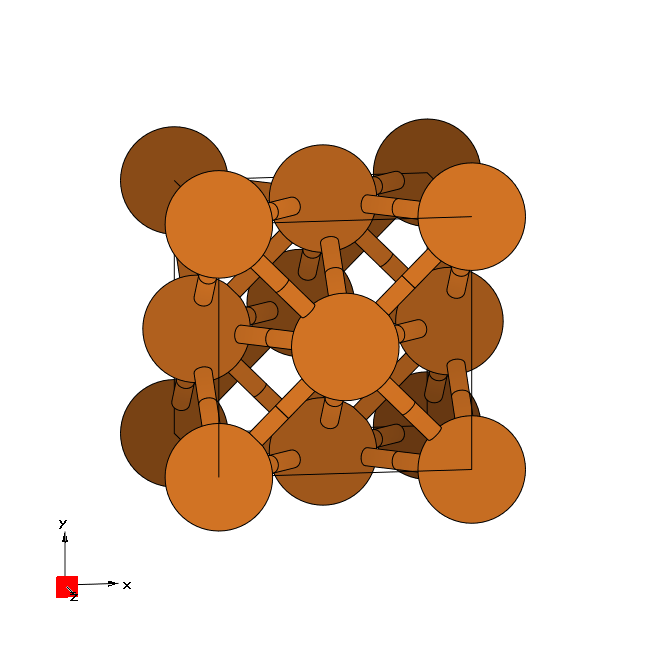
\includegraphics[width=0.25\columnwidth,trim={45pt 45pt 55pt 55pt},clip]{figure/example04/copper_crystal.png}
\caption{Unit cell of Copper crystal.}
\label{fig22.0}
\end{figure}

{\it Each directory creates $s$-like symmetry-adapted Wannier function centered at different position on top
of atomic centered $d$-like Wannier functions.}

Below it is reported the README file from the example directory

\begin{tcolorbox}
{\footnotesize 
\begin{verbatim}
# Symmetry-adapted mode

Additional input in Cu.win file 
  site_symmetry = .true.   (default value is .false.) 
  symmetrize_eps = 1d-9    (default value is 1d-3   )


Additional input in Cu.pw2wan file 
  write_dmn = .true.


Working directories 
  s_at_0.00 : s-like Wannier function centered at (0,0,0)       + atomic-centered d-like WFs  
  s_at_0.25 : s-like Wannier function centered at (1/4,1/4,1/4) + atomic-centered d-like WFs  
  s_at_0.50 : s-like Wannier function centered at (1/2,1/2,1/2) + atomic-centered d-like WFs 



In s_at_0.25, we use an additional flag "read_sym = .true." to customize the symmetry operations 
to be used.  
We exclude the inversion symmetry to create s-like Wannier function centered at (1/4,1/4,1/4). 
Information on symmetry operations without inversion symmetry is taken from GaAs calculation. 
See more detailed discussion in R. Sakuma, Phys. Rev. B 87, 235109 (2013). 
\end{verbatim}
}
\end{tcolorbox}

\clearpage
The space group of Cu is $Fm{-}3m$ (sequential  number 225 in the International Tables for Crystallography, Vol. A).


\subsection*{$s$-like Wannier function centred at the origin}
\begin{itemize}
	\item [1-5] {\it Compute the symmetry-adapted MLWFs.}

	In this example both the $s$-orbital and $d$-orbitals is placed at the origin, whose Wyckoff letter is $a$ and its multiplicity is $4$. The site symmetry group of $a$ is $m{-}3m$, which is isomorphous to the full point group of the crystal, known as $O_h$ and it contains 48 symmetry operations.
    The six \MLWFs{} obtained by placing both the initial $s$-orbital and the $d$-orbitals on the Cu atom are shown in \Fig{fig22.1}.
\end{itemize}

	\begin{figure}[h!]
	\centering
	\subfloat[$s$-like WF]{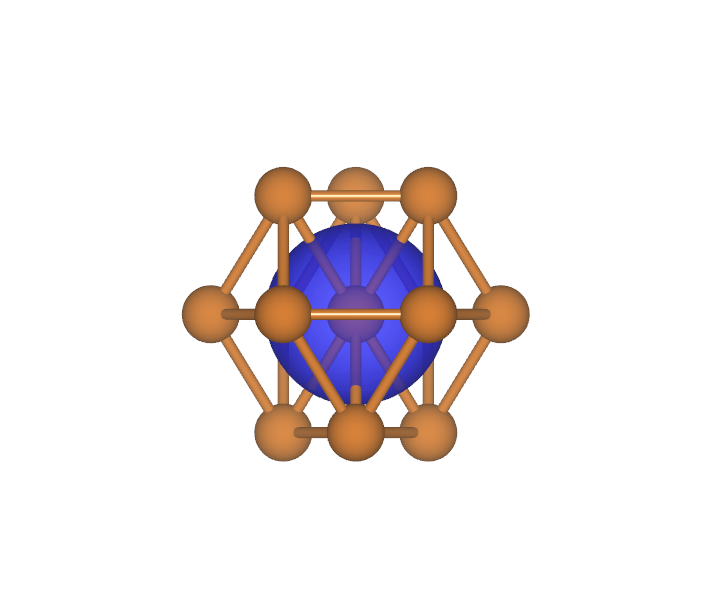
\includegraphics[width=0.15\columnwidth,trim={160pt 0pt 100pt 30pt},clip,rotate=-0.8]{figure/example22/Cu_000_s.png}}
	\centering
	\subfloat[$e_{g}$-like WF]{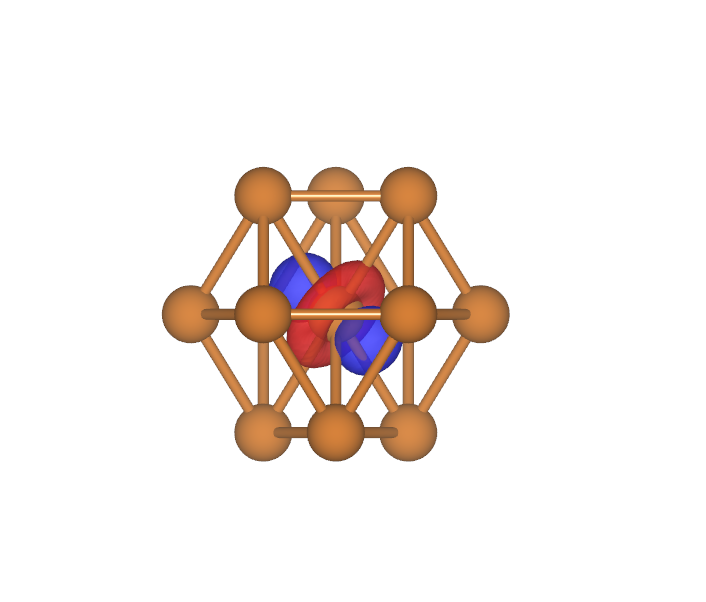
\includegraphics[width=0.15\columnwidth,trim={160pt 0pt 100pt 30pt},clip,rotate=-0.8]{figure/example22/Cu_000_d1.png}}
	\centering
	\subfloat[$e_{g}$-like WF]{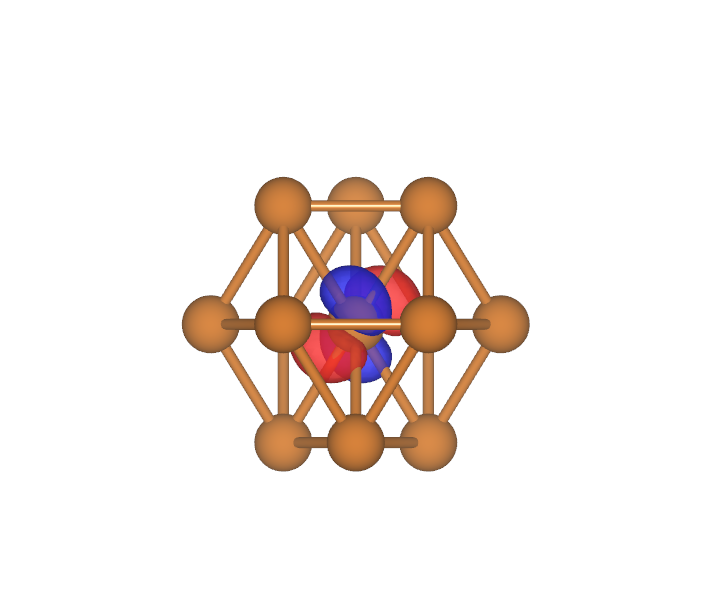
\includegraphics[width=0.15\columnwidth,trim={160pt 0pt 100pt 30pt},clip,rotate=-0.8]{figure/example22/Cu_000_d4.png}}\\
	\centering
	\subfloat[$t_{2g}$-like WF]{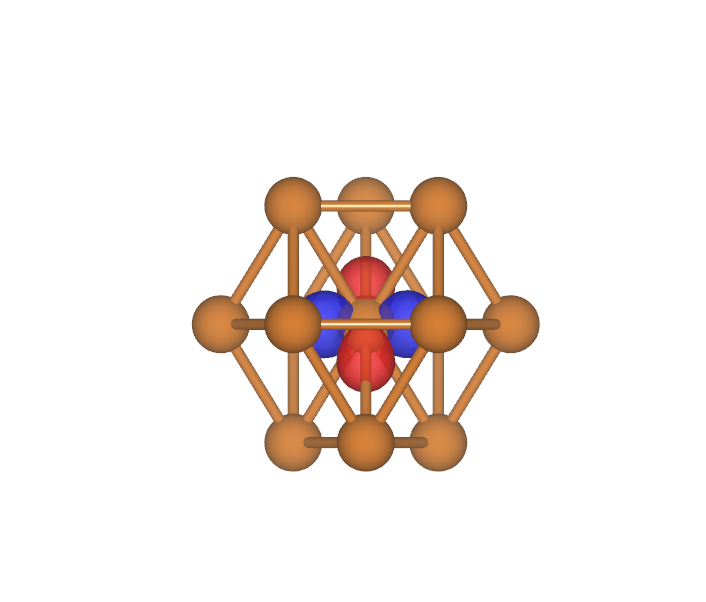
\includegraphics[width=0.15\columnwidth,trim={160pt 0pt 100pt 30pt},clip,rotate=-0.8]{figure/example22/Cu_000_d3.png}}
	\centering
	\subfloat[$t_{2g}$-like WF]{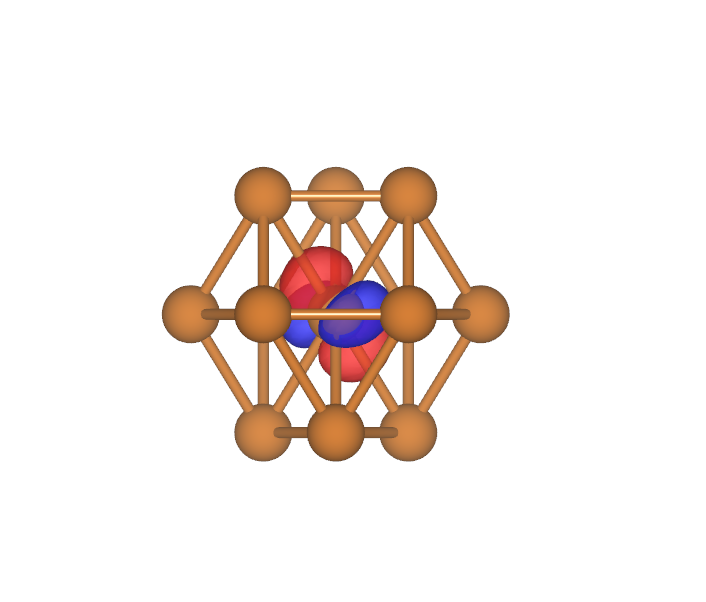
\includegraphics[width=0.15\columnwidth,trim={160pt 0pt 100pt 30pt},clip,rotate=-0.8]{figure/example22/Cu_000_d2.png}}
	\centering
	\subfloat[$t_{2g}$-like WF]{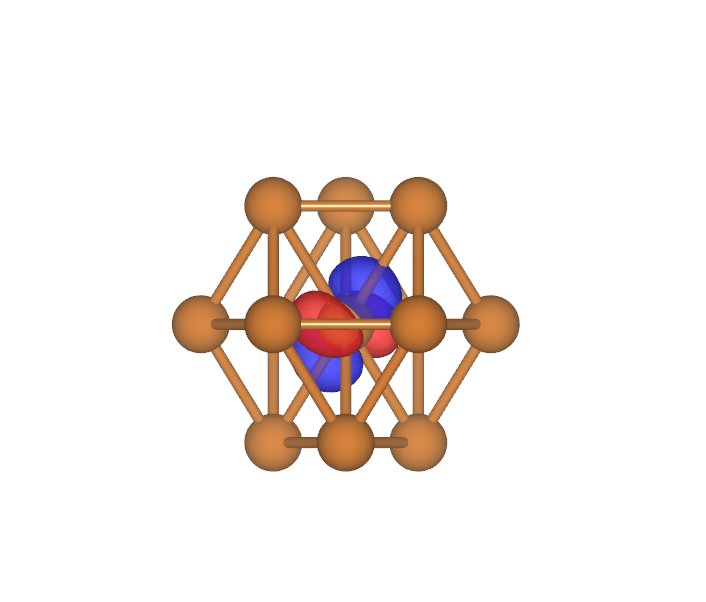
\includegraphics[width=0.15\columnwidth,trim={160pt 0pt 100pt 30pt},clip,rotate=-0.8]{figure/example22/Cu_000_d5.png}}
	\caption{Six symmetry-adapted \MLWFs{} in Cu. The initial $s$-orbital is placed at the origin.}
	\label{fig22.1}
	\end{figure}
\clearpage

\subsection*{$s$-like Wannier function centred at (0.25,0.25,0.25)}
\begin{itemize}
	\item [1-5] {\it Compute the symmetry-adapted MLWFs.}
	In this example the $s$-orbital is placed at (0.25,0.25,0.25), whose Wyckoff letter is $c$ and its multiplicity is $8$. The site symmetry group of $c$ is ${-}43m$, which is not isomorphous to the full point group of the crystal ($O_h$). This site symmetry group contains only 24 symmetry operations, \ie{} it comes from $O_h$ when inversion is removed. This is the reason why the flag {\tt read\_sym =.true. } in the {\tt .pw2wan} file and an additional input is required, namely {\tt Cu.sym}. In fact, this file is not automatically generated by {\tt pw2wannier90.x} but is given as input to be read.
    The six \MLWFs{} obtained by placing the initial $s$-orbital at (0.25,0.25,0.25) and the $d$-orbitals on the Cu atom are shown in \Fig{fig22.2}.  
\end{itemize}

	\begin{figure}[h!]
	\centering
	\subfloat[$s$-like WF]{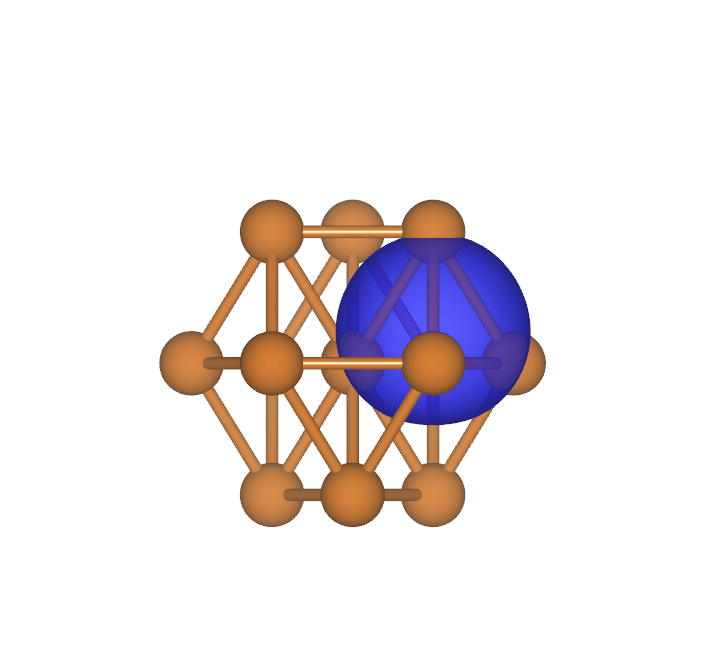
\includegraphics[width=0.15\columnwidth,trim={160pt 0pt 100pt 30pt},clip,rotate=-0.8]{figure/example22/Cu_025_s.png}}
	\centering
	\subfloat[$e_{g}$-like WF]{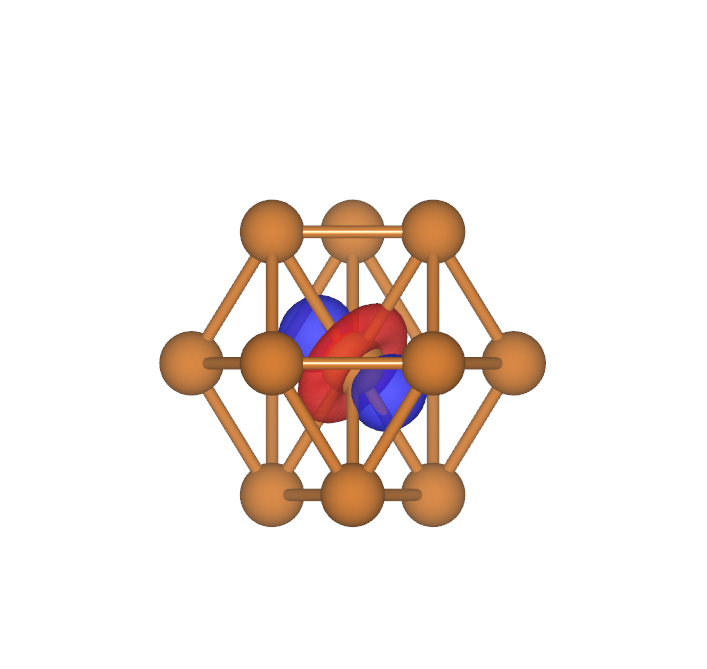
\includegraphics[width=0.15\columnwidth,trim={160pt 0pt 100pt 30pt},clip,rotate=-0.8]{figure/example22/Cu_025_d1.png}}
	\centering
	\subfloat[$e_{g}$-like WF]{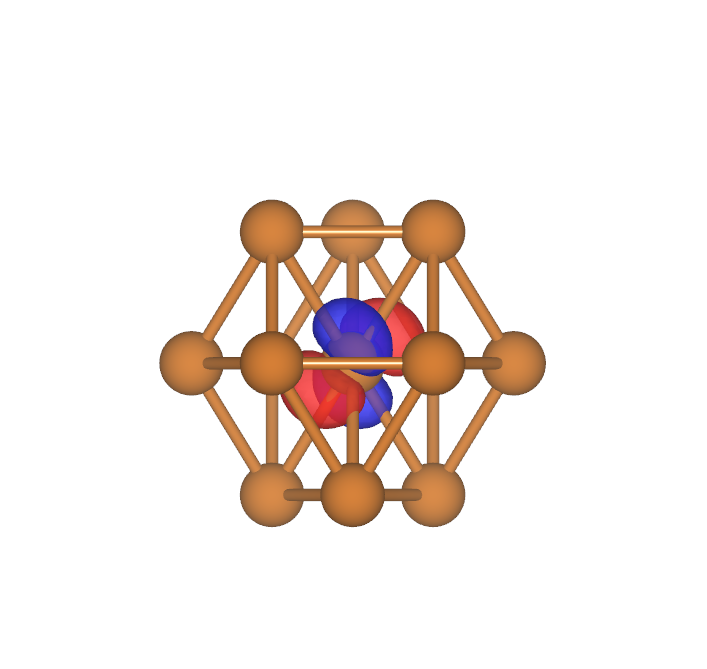
\includegraphics[width=0.15\columnwidth,trim={160pt 0pt 100pt 30pt},clip,rotate=-0.8]{figure/example22/Cu_025_d4.png}}\\
	\centering
	\subfloat[$t_{2g}$-like WF]{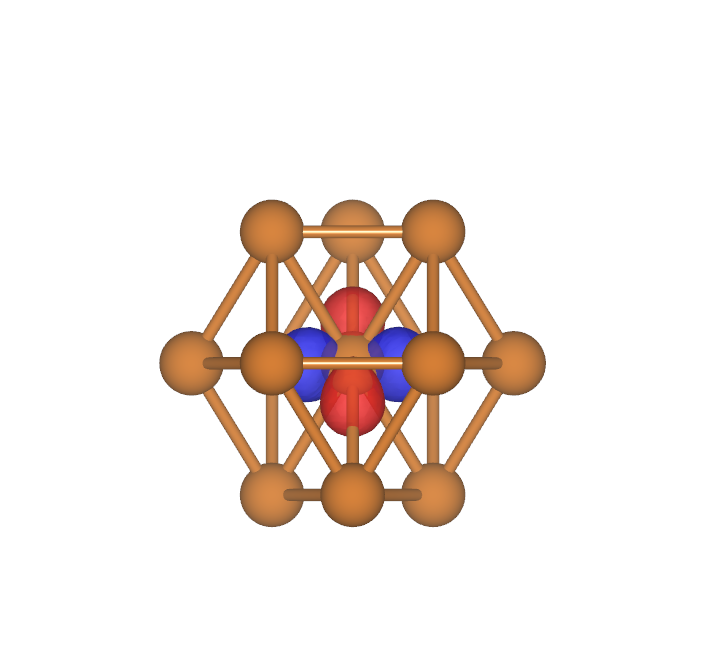
\includegraphics[width=0.15\columnwidth,trim={160pt 0pt 100pt 30pt},clip,rotate=-0.8]{figure/example22/Cu_025_d3.png}}
	\centering
	\subfloat[$t_{2g}$-like WF]{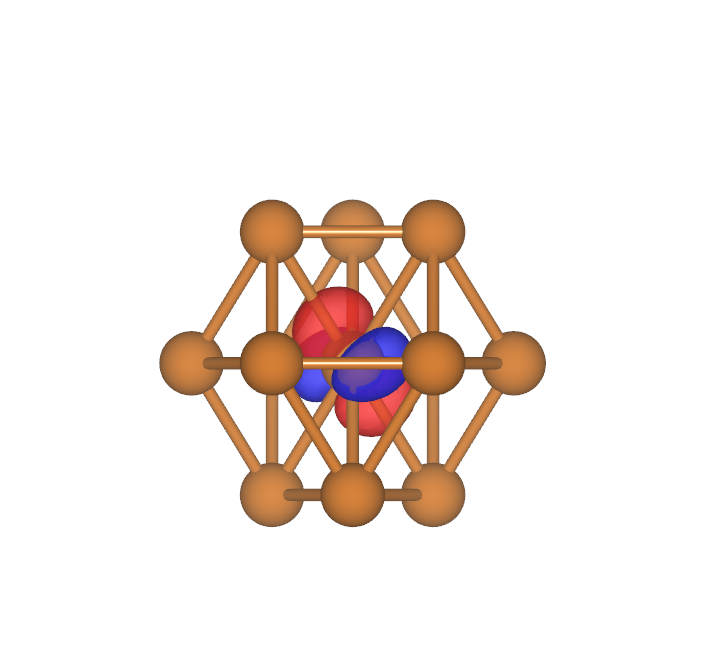
\includegraphics[width=0.15\columnwidth,trim={160pt 0pt 100pt 30pt},clip,rotate=-0.8]{figure/example22/Cu_025_d2.png}}
	\centering
	\subfloat[$t_{2g}$-like WF]{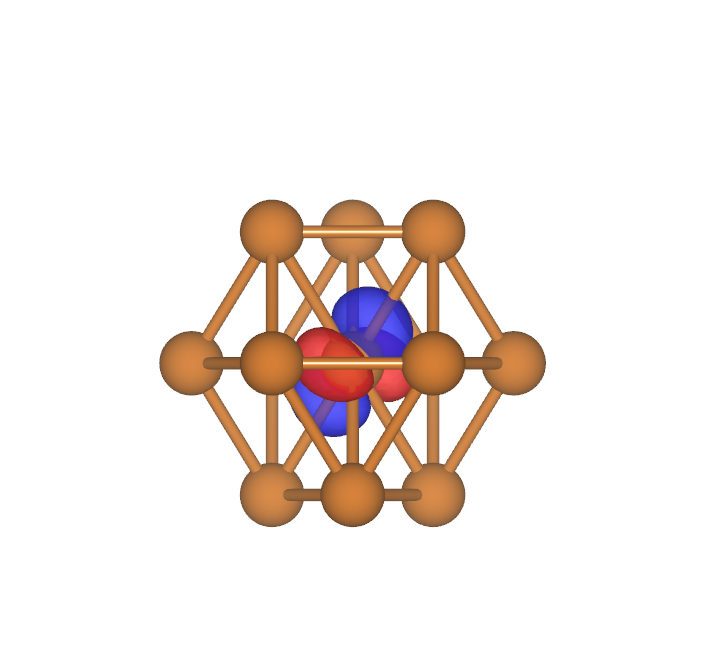
\includegraphics[width=0.15\columnwidth,trim={160pt 0pt 100pt 30pt},clip,rotate=-0.8]{figure/example22/Cu_025_d5.png}}
	\caption{Six symmetry-adapted \MLWFs{} in Cu. The initial $s$-orbital is placed at (0.25,0.25,0/25).}
	\label{fig22.2}
	\end{figure}
\clearpage

\subsection*{$s$-like Wannier function centred at (0.5,0.5,0.5)}
\begin{itemize}
	\item [1-5] {\it Compute the symmetry-adapted MLWFs.}
	In this example the $s$ orbital is placed at (0.5,0.5,0.5), whose Wyckoff letter is $b$ and its multiplicity is $4$. The site symmetry group of $c$ is $m{-}3m$, which is  isomorphous to the full point group of the crystal ($O_h$). Hence, no additional input file is needed in this case.
	The six \MLWFs{} obtained by placing the initial $s$-orbital at (0.5,0.5,0.5) and the $d$-orbitals on the Cu atom are shown in \Fig{fig22.3}.  	
\end{itemize}
\begin{figure}[h!]
	\centering
	\subfloat[$s$-like WF]{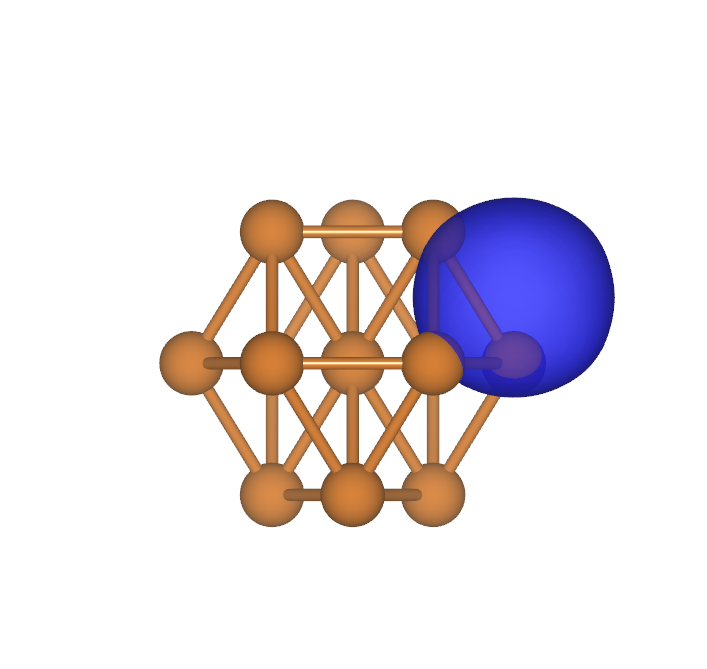
\includegraphics[width=0.15\columnwidth,trim={160pt 0pt 80pt 30pt},clip,rotate=-0.8]{figure/example22/Cu_05_s.png}}
	\centering
	\subfloat[$e_{g}$-like WF]{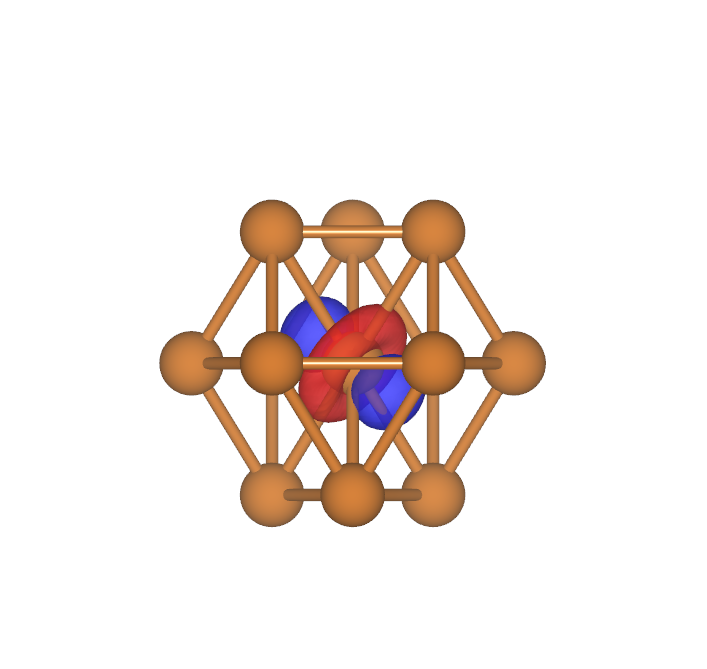
\includegraphics[width=0.15\columnwidth,trim={160pt 0pt 100pt 30pt},clip,rotate=-0.8]{figure/example22/Cu_05_d1.png}}
	\centering
	\subfloat[$e_{g}$-like WF]{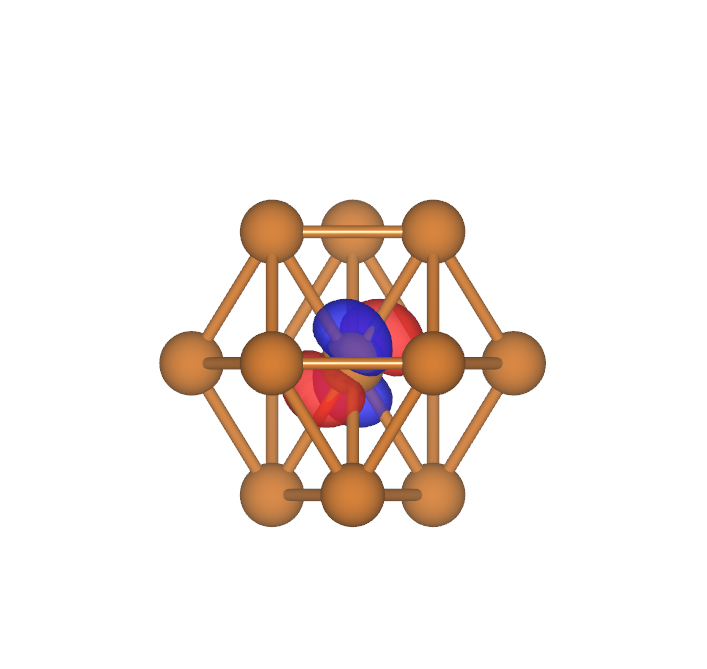
\includegraphics[width=0.15\columnwidth,trim={160pt 0pt 100pt 30pt},clip,rotate=-0.8]{figure/example22/Cu_05_d4.png}}\\
	\centering
	\subfloat[$t_{2g}$-like WF]{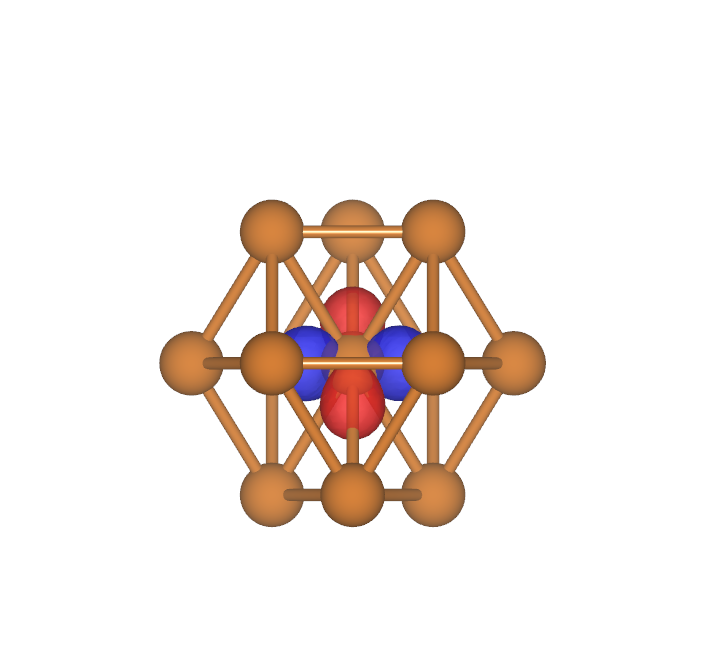
\includegraphics[width=0.15\columnwidth,trim={160pt 0pt 100pt 30pt},clip,rotate=-0.8]{figure/example22/Cu_05_d3.png}}
	\centering
	\subfloat[$t_{2g}$-like WF]{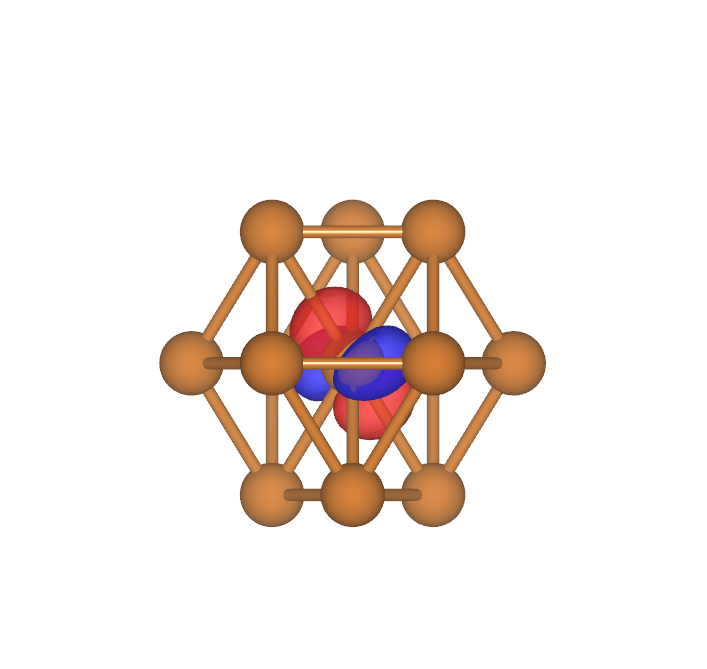
\includegraphics[width=0.15\columnwidth,trim={160pt 0pt 100pt 30pt},clip,rotate=-0.8]{figure/example22/Cu_05_d2.png}}
	\centering
	\subfloat[$t_{2g}$-like WF]{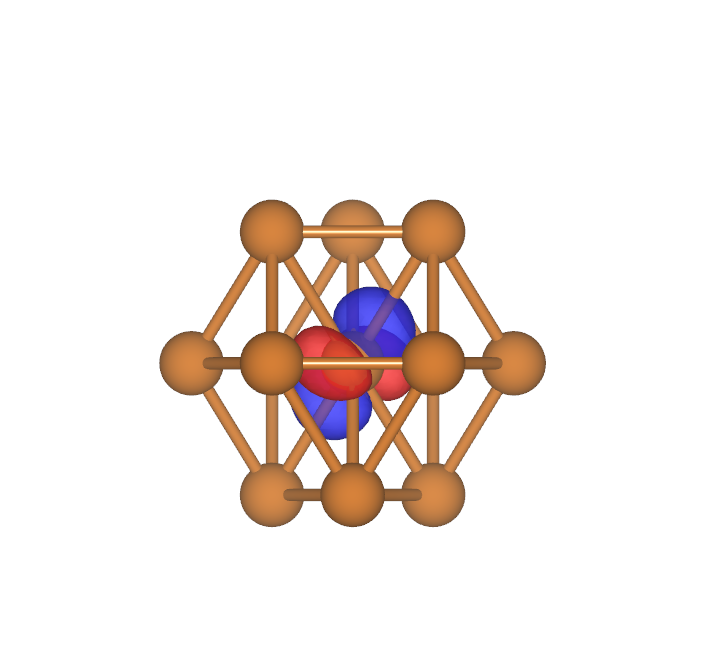
\includegraphics[width=0.15\columnwidth,trim={160pt 0pt 100pt 30pt},clip,rotate=-0.8]{figure/example22/Cu_05_d5.png}}
	\caption{Six symmetry-adapted \MLWFs{} in Cu. The initial $s$-orbital is placed at (0.5,0.5,0.5).}
	\label{fig22.3}
	\end{figure}
